\documentclass{rtxreport}

\author{Thomas Luquet}

\title{Bilan Architecture}

\rtxdoctype{Bilan Architecture}
\rtxdocref{2012\_AA2\_FR\_Rathaxes}
\rtxdocversion{1.0}
\rtxdocstatus{Finale}

\rtxdochistory{
0.1 & 16/11/2010 & Thomas Luquet & Premier draft \\
\hline
0.2 & 17/11/2010 & Louis Opter & Fixe compilation \\
\hline
0.3 & 17/11/2010 & Louis Opter & Ajout du cartouche \\
\hline
0.4 & 17/11/2010 & David Pineau & Complétion de la section Technologie \\
\hline
0.5 & 17/11/2010 & Louis Opter & Reformulations et ajout de notes \\
\hline
0.6 & 17/11/2010 & Thomas Luquet & Reformulations, insertion des graphiques \\
\hline
0.7 & 17/11/2010 & Luquet Thomas & Reformulations, corrections diverses \\
\hline
0.8 & 17/11/2010 & Louis Opter & Relecture et corrections \\
\hline
0.9 & 16/12/2010 & Louis Opter & Copie à partir de AA1 \\
\hline
1.0 & 16/12/2010 & Louis Opter & Prise en compte des critiques faites sur l'AA1 \\
\hline
1.1 & 04/02/2011 & David Pineau & Correction de la section fonctionnelle détaillée selon les évolutions du projet \\
\hline
1.2 & 09/02/2011 & David Pineau & Ajout d'un logigramme décrivant le fonctionnement du compilateur \\
}

\newcommand{\note}[1]{\marginpar{\scriptsize{\textdagger\ #1}}}

\begin{document}

\maketitle

\rtxmaketitleblock

\tableofcontents

\chapter{Rappel du projet}

\section{Qu'est ce que \rtx\ ?}

\rtx\ est un ensemble d'outils permettant de simplifier l'écriture de pilote de
périphérique. Le projet permet de générer un code source écrit en C pour Linux,
Windows 7 et OpenBSD à partir d'un fichier de description de pilote.

Le projet \rtx\ 2012 est une amélioration de l'EIP réalisé en 2009. Il
incorpore de nouvelles fonctionnalitées comme l’asynchronicité. \rtx\ 2012 sera
capable de générer un pilote de souris USB et celui d'une carte son qui
serviront à prouver que le concept fonctionne.

Nous ciblons la communauté scientifique et nous avons décidé de rendre le
développement du projet publique grâce à un dépôt Google
code\footnote{\url{http://code.google.com/p/rathaxes/}} et des licences libres.

\section{Structure du projet}

% Ne pas dire Rathaxes ici car juste en dessous on dit que c'est un
% compilateur…
Le projet est divisé en trois parties :
\begin{enumerate}
\item Le langage \rtx\ : un langage dédié (DSL\footnote{Domain Specific
Language.}) utilisé pour décrire un pilote~;
\item La \BL: Elle permet l'interfaçage entre le DSL et le compilateur~;
\item Le compilateur : Il transforme les fichiers \rtx\ (\texttt{.rtx}) ---à
l'aide de la \BL--- en fichier \texttt{.c} spécifiques au système d'exploitation
choisi.
\end{enumerate}

La \BL\ et nos documentations constituent notre base de données.

\chapter{Diagrammes}

\section{Description fonctionnelle}

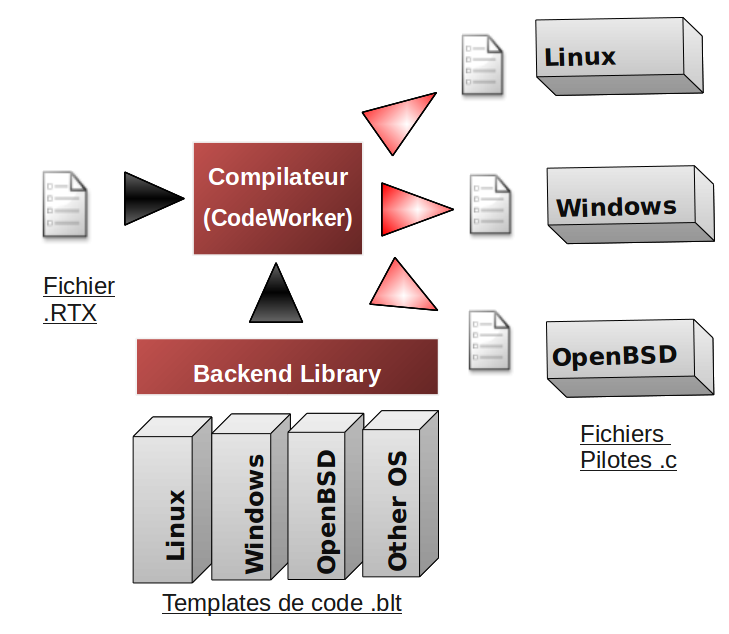
\includegraphics[width=0.95\textwidth]{diagramme_general}

\rtx\ utilise le langage CodeWorker\cite{CodeWorker} pour l'analyse du DSL ainsi
que la génération d'un AST\footnote{Abstract Syntax Tree: Arbre de Syntaxe
Abstraite.}. Enfin, CodeWorker utilise cet AST, pour générer le code C du
driver. Afin de pouvoir générer du code C à partir du DSL de \rtx, le
compilateur utilise une bibliothèque de modèles appelé \BL.

\section{Diagramme détaillé}

\subsection{Les composants du compilateur}

Actuellement le compilateur \rtx\ de la promotion 2009 fonctionne ainsi~:
\begin{enumerate}
\item Il transforme les fichier \texttt{.rtx} (écrit dans le DSL \rtx) en un AST~;
\item Il parcourt cet arbre. En fonction des mots clefs rencontrés, le
compilateur sélectionne des fichiers BLT issus de la \BL~;
\item Enfin il génère des fichiers de pilote de périphérique selon l'arbre
reconstruit à partir des modèles de la BLT.
\end{enumerate}

Notre objectif est de modifier le comportement du compilateur dans le but de
rendre les modifications futures du langage plus simples à implémenter.
Nous pourrons ainsi identifier les éléments principaux du compilateur comme
suit :

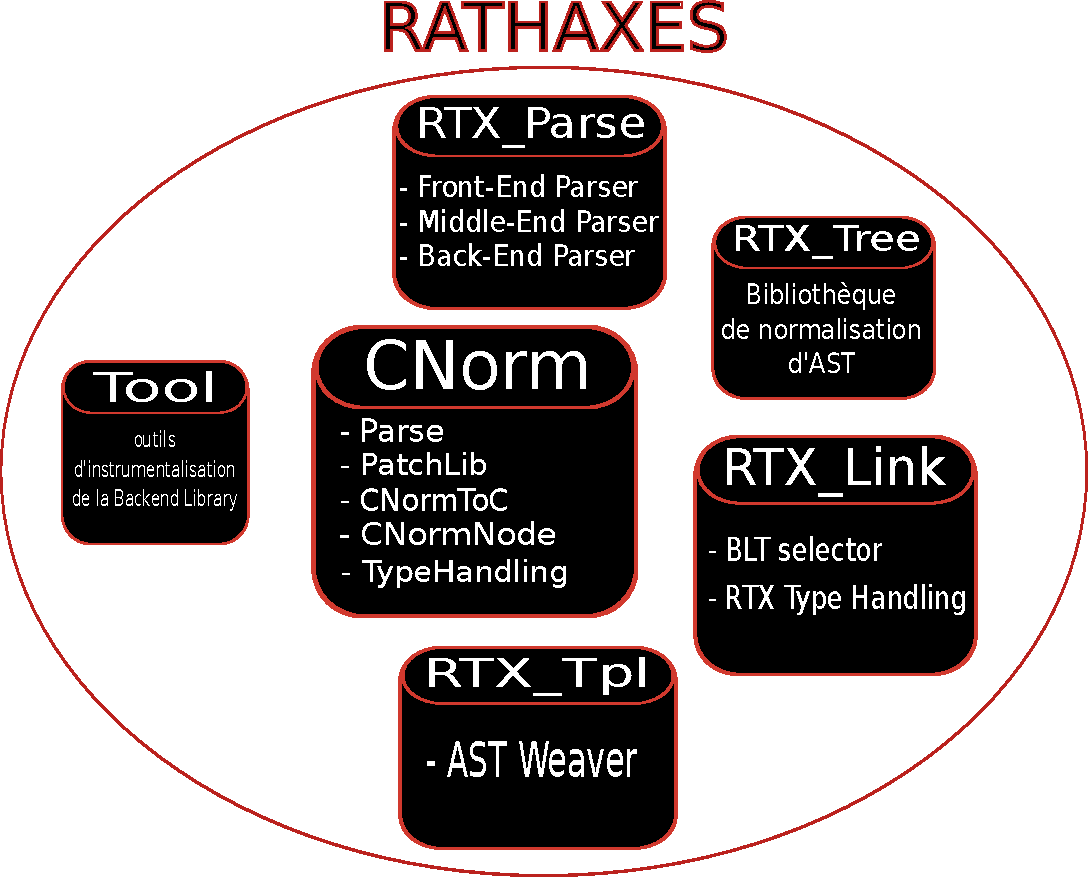
\includegraphics[width=0.95\textwidth]{diagramme_architecture.pdf}

On constate donc plusieurs éléments qui se démarquent les uns des
autres au sein du compilateur, chacun ayant son rôle défini :
\begin{itemize}
\item CNorm : bibliothèque externe se chargeant de tout code relevant du
        langage C. Elle contient :
        \begin{itemize}
        \item Parse : élément chargé de construire un AST à
                partir de code source C ;
        \item PatchLib : ensemble de fonctionnalités permettant de manipuler
                et d'annoter un AST ;
        \item CNormToC : élément générant du code C à partir
                d'un AST ;
        \item CNormNode : bibliothèque de normalisation d'AST ;
        \item TypeHandling : élément se chargeant de vérifier la
                validité des expressions contenues dans un AST ;
        \end{itemize}
\item Tool : suite d'outils permettant d'instrumentaliser la manipulation de
        l'AST généré par RTX\_Parse ;
\item RTX\_Parse : élément chargé de construire un AST à partir
        de n'importe quelle partie du DSL (Front-end, Middle-end ou Back-end) ;
\item RTX\_Tree : bibliothèque de normalisation d'AST pour rathaxes ;
\item RTX\_Link : élément sélectionnant des modèles de code
        à instancier, selon les informations contenues dans l'AST actuel et
        effectue les vérifications de validité des expressions contenues
        dans l'AST ;
\item RTX\_Tpl : ensemble d'outils permettant d'instrumenter le tissage de
        plusieurs AST entre eux. Cela permettra à terme d'intégrer du
        code C au sein des modèles de code de manière simplifiée.
\end{itemize}

Pour cette raison, plusieurs éléments du compilateur vont changer
fondamentalement :
\begin{itemize}
\item Conception du langage Rathaxes ;
\item Approche de la construction de l'Arbre de Syntaxe Abstraite final.
\end{itemize}

Commençons par la conception que nous avons du langage Rathaxes
lui-même. L'équipe 2009 visualisait le \emph{DSL} du \emph{Front-end},
contenu dans les fichiers \texttt{.rtx} comme un language tout à fait
distinct du language présent dans les fichiers \texttt{.rtx} du
\emph{Back-end}. Désormais, aussi bien du point de vue du compilateur que
du point de vue d'un utilisateur, nous désirons que le \emph{Front-end} et
le \emph{Back-end} de Rathaxes soit un seul et même language. On pourra
aussi constater l'apparition d'un \emph{Middle-end}, correspondant plutôt
à la partie du language \emph{interne} au compilateur. Y seront liés
notamment les différents builtins que celui-ci comportera.

De plus, la construction de l'Arbre de Syntaxe Abstraite va être
découpée de manière beaucoup plus claire et explicite au sein du
compilateur.
En effet, jusqu'à maintenant, le code que l'on pouvait écrire dans un
fichier \texttt{.rtx} dépendait de ce qui était implémenté au
niveau des modèles de code, les fichier \texttt{.blt}. Nous souhaitons
alléger cette relation entre \emph{Front-end} et \emph{Back-end}, en
normalisant le langage, ce qui nous permettra non seulement de le documenter
plus facilement, mais aussi de rendre ces deux parties quasi-indépendantes.

\subsection{Logigramme d'exécution}

Le flux d'entrée de Rathaxes, selon les mots clefs qu'il contient,
pourra être traité différemment qu'il l'est actuellement.
Le schéma ci-dessous détaille ce processus de génération de code source
\texttt{.c} à partir d'un fichier \texttt{.rtx} passé en entrée du
compilateur.

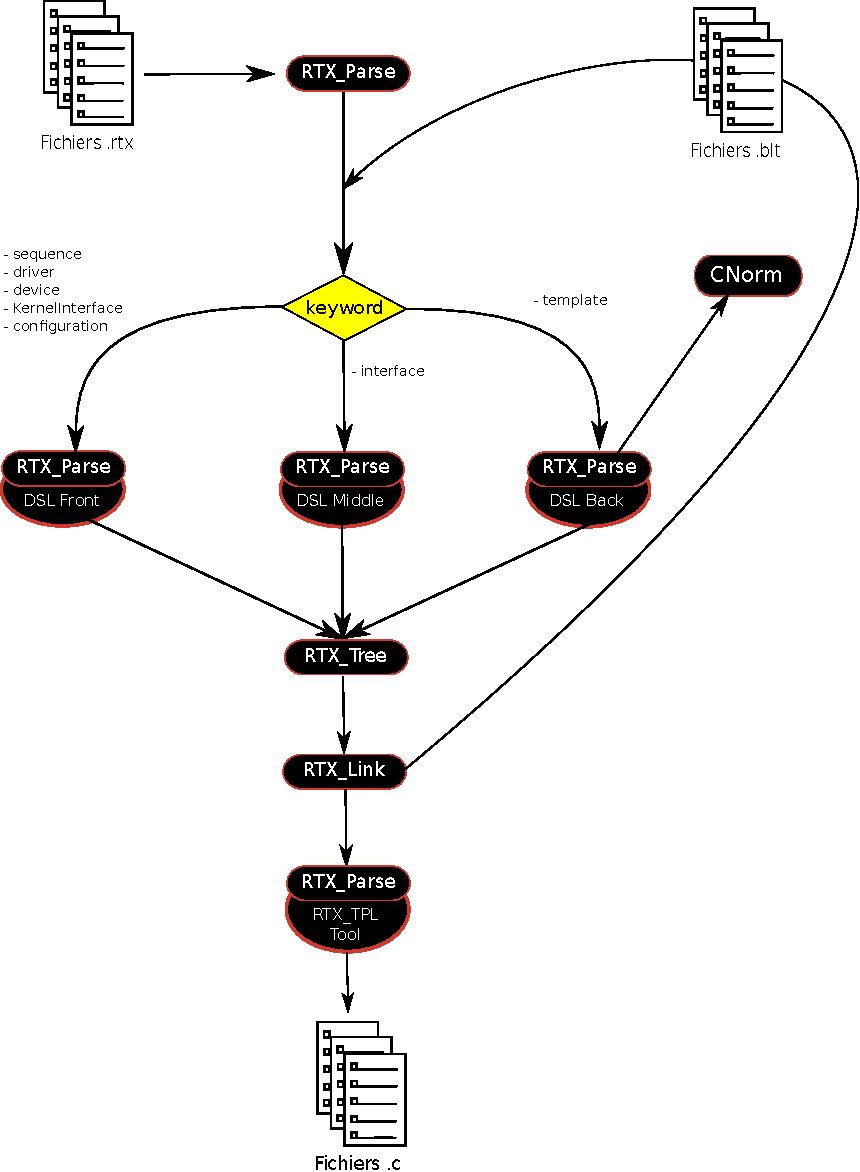
\includegraphics[width=0.95\textwidth]{logigramme.pdf}

Le premier élément entrant en jeu dans le compilateur sera  RTX\_Parse.
Celui-ci, en fonction du mot-clef identifié, fera appel aux fonctionnalités
d'analyse syntaxique du Front-end (contenu usuel d'un fichier \texttt{.rtx}),
du Middle-end (fonctionnement interne du compilateur), ou du Back-end
(contenu usuel d'un fichier \texttt{.blt}). Dans le cas d'un mot-clef dirigeant
l'analyse syntaxique du flux vers l'élément Back-end de RTX\_Parse, il est
possible que le CNorm soit directement utilisé, puisque cette partie du langage
prévoit d'embarquer du code C.

L'arbre de syntaxe abstraite(\emph{AST}) généré par RTX\_Parse (quel que soit
l'élément réellement utilisé lors de l'analyse du fichier source), va tout
d'abord être transformé à l'aide de l'élément RTX\_Tree, afin de normaliser
sa structure.

Alors seulement, le composant RTX\_Link sera utilisé pour détecter et
sélectionner les fichiers \texttt{.blt} correspondant à des algorithmes et
des types contenus dans les fichiers \texttt{.rtx} sources. Chacun de ces
fichiers modèles va alors permettre de générer un \emph{AST}, qui sera par
la suite assemblé avec l'\emph{AST} principal généré lors de l'analyse des
fichiers \texttt{.rtx}.

Ces différents arbres seront donc assemblés a l'aide du composant
RTX\_TPL du compilateur. En effet, son rôle est de \emph{tisser} différents
arbres de syntaxe ensemble, en conservant les relations de type, et en
associant correctement les éléments des différents arbres, que ce soit des
types ou des algorithmes.

De plus, les différents outils contenus par Tool seront utilisés afin
de générer non seulement les fichiers \texttt{.c} mais aussi les éléments
nécessaires à la compilation et au bon fonctionnement du pilote résultant.
Par exemple, dans le cas de Windows, des fichiers \texttt{.inf} sont requis
afin de charger le pilote dans le système d'exploitation. La génération de ce
type de fichier serait une des tâches du composant Tool.


\chapter{La technologie \rtx}

\section{Un héritage}

Un grand nombre de choix technologiques ont été effectués par l'équipe 2009.
Ils avaient besoin d'une technologie permettant d'implémenter facilement un
compilateur, qui puisse utiliser des modèles de code.

\subsection{Un compilateur}

Pour écrire le compilateur, l'outil retenu par la première équipe est
CodeWorker. CodeWorker est un langage interprété dont la syntaxe s'inspire la
notation EBNF\footnote{Extended Backus--Naur Form}. L'interpréteur CodeWorker
est distribué gratuitement sous la licence libre LGPL\cite{LGPL21}.

CodeWorker, présente l'avantage d'être facilement abordable et permet une
analyse syntaxique et lexicale avancée, tout en permettant la génération de
code en se basant sur l'arbre de syntaxe abstraite généré par le code
précédemment analysé.

De plus, la syntaxe proposée pour le langage de script de CodeWorker est pour
la partie analyse syntaxique relativement proche de la syntaxe EBNF. De même,
la syntaxe proposée pour le script de manipulation d'arbre syntaxique et de
génération est dérivée du C, la rendant relativement familière à l'ensemble de
l'équipe qui maitrise le C.

\subsection{Une série de modèles}

L'objectif du projet est de générer des drivers en C pour différents systèmes
d'exploitation. Ceci doit être fait en indépendance des connaissances
spécifiques à un OS. Il est donc nécessaire de posséder un système de modèles
de code utilisables pour générer du code C pour chaque système spécifique.

Ces modèles de code portent l'extension \texttt{.blt} pour \BL\ Template.

C'est aussi pour cela que l'équipe 2009 a choisi CodeWorker comme l'outil le plus
pratique. En effet, la solution la plus simple pour avoir des modèles de code
qui permettent de générer du code C est d'écrire directement des modèles
en script CodeWorker, de manière a réduire la quantité de travail nécessaire
du côté du backend de \rtx\ (pour la partie parsing).

\section{Un langage}

Forts de l'expérience acquise par l'équipe 2009 de \rtx, l'objectif de
notre groupe est de rechercher et implémenter de nouveaux concepts dans
\rtx. Parmi ceux-ci, s'illustre notamment les notions d'asynchronicité,
de DMA\footnote{Direct Memory Access.}, d'IRQ\footnote{Interrupt ReQuest.} et
enfin l'ensemble des concepts liés à l'utilisation de BUS tels que le PCI dans
les pilotes de périphériques.

Un autre objectif de notre équipe est d'apporter des améliorations dans le
fonctionnement même de \rtx. Jusqu'alors, le code C était généré par
activation des modèles en fonction du contenu de l'arbre de syntaxe abstraite.
Nous désirons changer cela, pour d'une part rendre le cœur du compilateur
plus générique, et permettre de tester efficacement chaque étape
d'implémentation du langage.

Pour cela, nous allons conserver le CodeWorker, qui par sa simplicité, nous
permettra de modifier le cœur du compilateur, afin par la suite de pouvoir
facilement intégrer de nouveaux concepts et mots clefs au compilateur. Par
ailleurs nous pourrons intégrer plus aisément des contributeurs externes au
projet.

\newpage

\rtxbibliography

\end{document}
